	\chapter*{Introduction}
	\addcontentsline{toc}{chapter}{Introduction}
	
	FTL : Faster than Light (\url{http://www.ftlgame.com/}) est un jeu de science fiction de Subset Games pour PC, mélangeant la gestion, la stratégie et le jeu de rôle à bord d'un vaisseau spatial. Le joueur a pour objectif de conduire son vaisseau d'un point A à un point B de la galaxie, tout en faisant face aux multiples situations qui se présentent à lui aléatoirement. Il doit ainsi survivre face à de nombreux événements : affronter des adversaires, négocier avec d'autres vaisseaux, échanger des ressources, acheter de l'équipement, etc. Le but est donc de rester le plus longtemps en vie pour aller le plus loin possible dans l'espace. Ainsi, le principe primaire du jeu est de s'adapter à un environnement hostile en optimisant son vaisseau, ses équipements (tels que des drônes ou de nombreuses armes), et son équipage qui est composé de plusieurs races possédants chacune des avantages et des inconvénients.
	\begin{figure}[H]
		\caption{Capture d'écran du jeu Faster Than Light}
		\label{fig:screen}
		\centering
		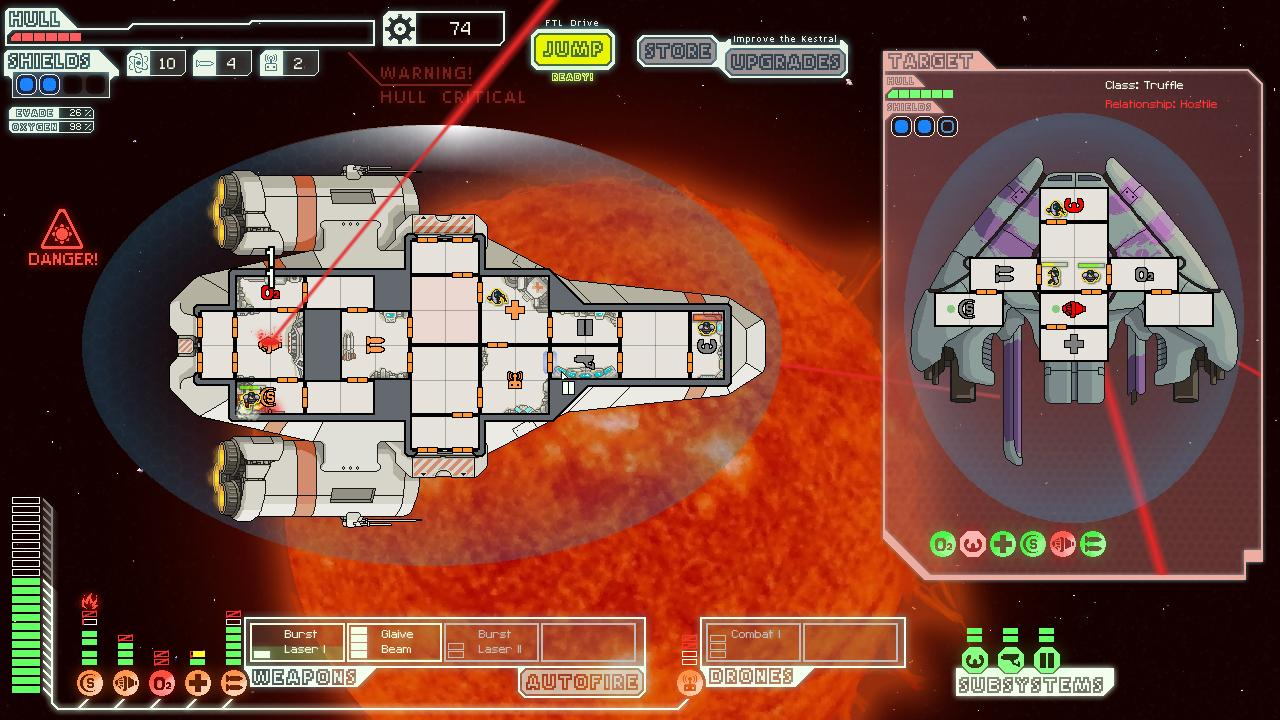
\includegraphics[width=1\linewidth]{screen.jpg}
	\end{figure}
	Ci-dessus (figure~\ref{fig:screen}), nous pouvons voir une capture d'écran du jeu Faster Than Light présentant un vaisseau durant un combat. Nous pouvons y observer la structure géographique d'un vaisseau, avec la distribution de l'énergie dans ses systèmes en bas à gauche.
	
	
	Au cours du premier semestre, nous avons réussi à réaliser un moteur de combat qui, même s'il n'est pas complet, se rapproche du jeu original, ce qui nous permet maintenant de finaliser notre projet : optimiser la recherche d'un vaisseau meilleur que les autres.
	
	
	L'objectif de ce semestre est donc de faire un programme qui détermine le meilleur vaisseau pour un coût maximal donné. Pour cela, on peut séparer le projet en deux parties : faire un générateur de vaisseaux selon un coût donné et faire un algorithme qui détermine le meilleur vaisseau.

	Dans ce rapport nous rappellerons le fonctionnement du moteur de combat qui a reçu quelques ajouts durant le second semestre. Ensuite, nous verrons en détail les techniques employées dans la construction de vaisseaux et la recherche du meilleur vaisseau. Enfin, nous pourrons parler de la construction du programme, étudier les résultats donnés par le programme et exprimer quelques critiques.
